
%(BEGIN_QUESTION)
% Copyright 2014, Tony R. Kuphaldt, released under the Creative Commons Attribution License (v 1.0)
% This means you may do almost anything with this work of mine, so long as you give me proper credit

Identify whether or not the HART communicator will be able to communicate with the HART transmitter in each of these circuits, explaining why or why not for each case:

\vskip 20pt

\noindent
{\bf Circuit \#1:}

$$\includegraphics[width=15.5cm]{i03332x01.eps}$$

\vskip 20pt
\noindent
{\bf Circuit \#2:}

$$\includegraphics[width=15.5cm]{i03332x02.eps}$$

\filbreak

\vskip 20pt
\noindent
{\bf Circuit \#3:}

$$\includegraphics[width=15.5cm]{i03332x03.eps}$$

\vskip 20pt
\noindent
{\bf Circuit \#4:}

$$\includegraphics[width=15.5cm]{i03332x04.eps}$$

\filbreak

\vskip 20pt
\noindent
{\bf Circuit \#5:}

$$\includegraphics[width=15.5cm]{i03332x05.eps}$$

\vskip 20pt
\noindent
{\bf Circuit \#6:}

$$\includegraphics[width=15.5cm]{i03332x06.eps}$$

\filbreak

\vskip 20pt
\noindent
{\bf Circuit \#7:}

$$\includegraphics[width=15.5cm]{i03332x07.eps}$$

\vskip 20pt
\noindent
{\bf Circuit \#8:}

$$\includegraphics[width=15.5cm]{i03332x08.eps}$$

\filbreak

\vskip 20pt
\noindent
{\bf Circuit \#9:}

$$\includegraphics[width=15.5cm]{i03332x09.eps}$$

\vskip 20pt
\noindent
{\bf Circuit \#10:}

$$\includegraphics[width=15.5cm]{i03332x10.eps}$$



\underbar{file i03332}
%(END_QUESTION)





%(BEGIN_ANSWER)

\noindent
{\bf Partial answer:}

\begin{itemize}
%\item{} Circuit \#1: {\bf Yes}
\item{} Circuit \#2: {\bf Yes}
\item{} Circuit \#3: {\bf No}
%\item{} Circuit \#4: {\bf No}
%\item{} Circuit \#5: {\bf No}
\item{} Circuit \#6: {\bf Yes}
%\item{} Circuit \#7: {\bf Yes}
%\item{} Circuit \#8: {\bf Yes}
\item{} Circuit \#9: {\bf No}
%\item{} Circuit \#10: {\bf No}
\end{itemize}

Hint: apply the Superposition Theorem to each circuit example, where the HART communicator is the only active signal source in the circuit, and see if the communicator's signal is able to reach the transmitter.

%(END_ANSWER)





%(BEGIN_NOTES)

\begin{itemize}
\item{} Circuit \#1: {\bf Yes}
\item{} Circuit \#2: {\bf Yes}
\item{} Circuit \#3: {\bf No}
\item{} Circuit \#4: {\bf No} (the resistor here does {\it nothing} useful!
\item{} Circuit \#5: {\bf No}
\item{} Circuit \#6: {\bf Yes}
\item{} Circuit \#7: {\bf Yes}
\item{} Circuit \#8: {\bf Yes}
\item{} Circuit \#9: {\bf No}
\item{} Circuit \#10: {\bf No}
\end{itemize}

In each case, if we replace the batteries (voltage source) with a short-circuit to represent their internal resistances, we see that the HART communicator's signal will become shorted out by the batteries in all the non-working cases.





\vfil \eject

\noindent
{\bf Summary Quiz:}

Asking students to explain whether or not these HART circuits will communicate is a good summary quiz, especially if you require they apply the Superposition Theorem as part of their analyses.

%INDEX% Fieldbus, HART: analysis of 4-20 mA / HART transmitter circuit using Superposition Theorem
%INDEX% Fieldbus, HART: transmitter circuit

%(END_NOTES)

